\documentclass[11pt,a4paper]{article}

\usepackage[utf8]{inputenc}
\usepackage[T1]{fontenc}
\usepackage{amsmath}
\usepackage{tikz}
\usepackage{pgfplots}

\pgfplotsset{compat=1.18}
\usetikzlibrary{calc, positioning, arrows.meta, shapes.geometric}
\usepgfplotslibrary{fillbetween}

\title{TikZ and PGFPlots Stress Document}
\author{OverBranch Benchmark Corpus}
\date{}

\begin{document}

\maketitle

\section{Function plot}

The plot below samples a damped oscillation densely, which makes it a
useful workload for measuring the cost of PGFPlots evaluation.

\begin{center}
  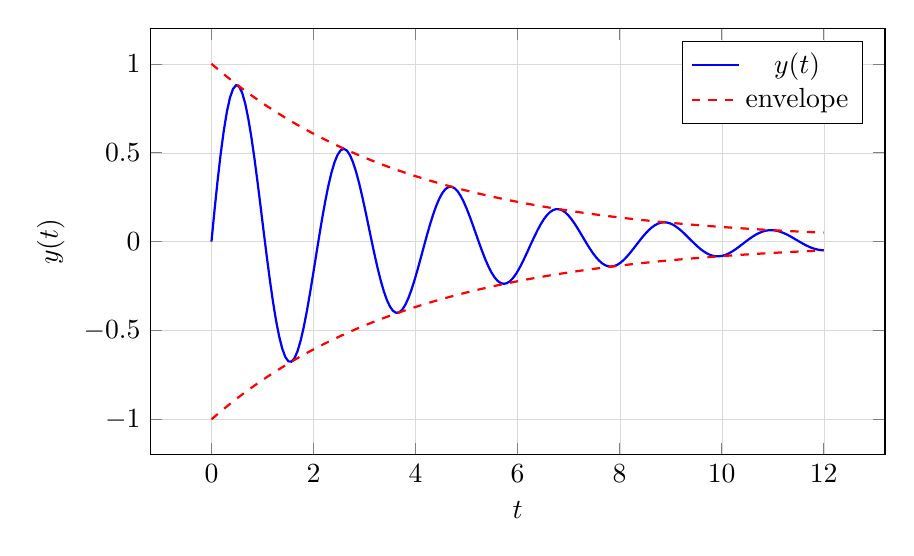
\begin{tikzpicture}
    \begin{axis}[
        width=0.9\textwidth, height=7cm,
        xlabel={$t$}, ylabel={$y(t)$},
        domain=0:12, samples=200,
        grid=both, grid style={line width=.1pt, draw=gray!30},
        legend pos=north east,
      ]
      \addplot[blue, thick] {exp(-0.25*x)*sin(deg(3*x))};
      \addplot[red, dashed, thick] {exp(-0.25*x)};
      \addplot[red, dashed, thick, forget plot] {-exp(-0.25*x)};
      \legend{$y(t)$, envelope}
    \end{axis}
  \end{tikzpicture}
\end{center}

\section{Bar chart}

\begin{center}
  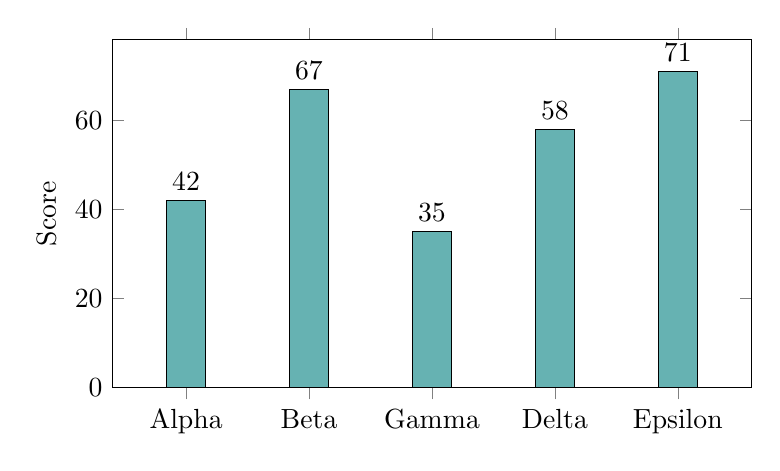
\begin{tikzpicture}
    \begin{axis}[
        ybar, bar width=14pt,
        width=0.8\textwidth, height=6cm,
        symbolic x coords={Alpha, Beta, Gamma, Delta, Epsilon},
        xtick=data, nodes near coords, ymin=0,
        ylabel={Score}, enlarge x limits=0.15,
      ]
      \addplot[fill=teal!60] coordinates {(Alpha,42) (Beta,67) (Gamma,35) (Delta,58) (Epsilon,71)};
    \end{axis}
  \end{tikzpicture}
\end{center}

\section{Surface plot}

\begin{center}
  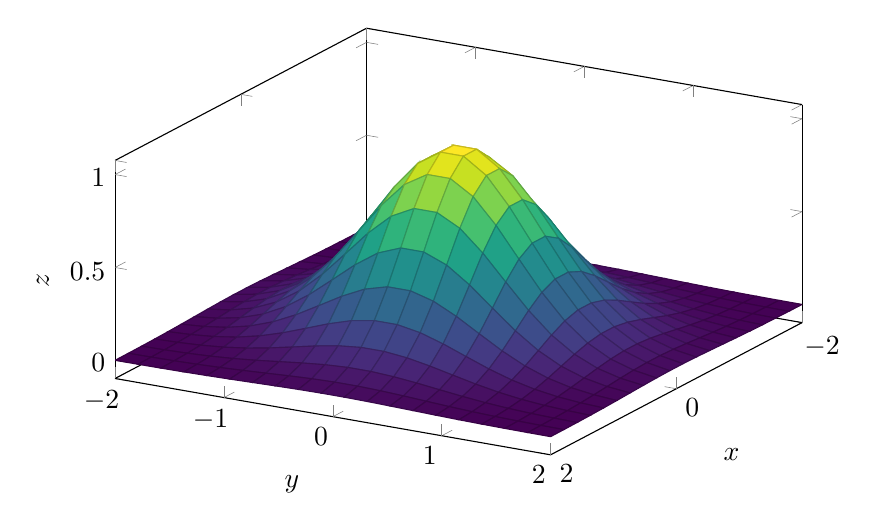
\begin{tikzpicture}
    \begin{axis}[
        view={120}{35}, width=0.85\textwidth, height=7cm,
        xlabel={$x$}, ylabel={$y$}, zlabel={$z$},
        domain=-2:2, y domain=-2:2, samples=20, samples y=20,
        colormap/viridis,
      ]
      \addplot3[surf] {exp(-x^2-y^2)};
    \end{axis}
  \end{tikzpicture}
\end{center}

\section{Flowchart}

The flowchart uses \texttt{positioning} for layout, \texttt{shapes.geometric}
for the node shapes, and \texttt{arrows.meta} for the edges.

\begin{center}
  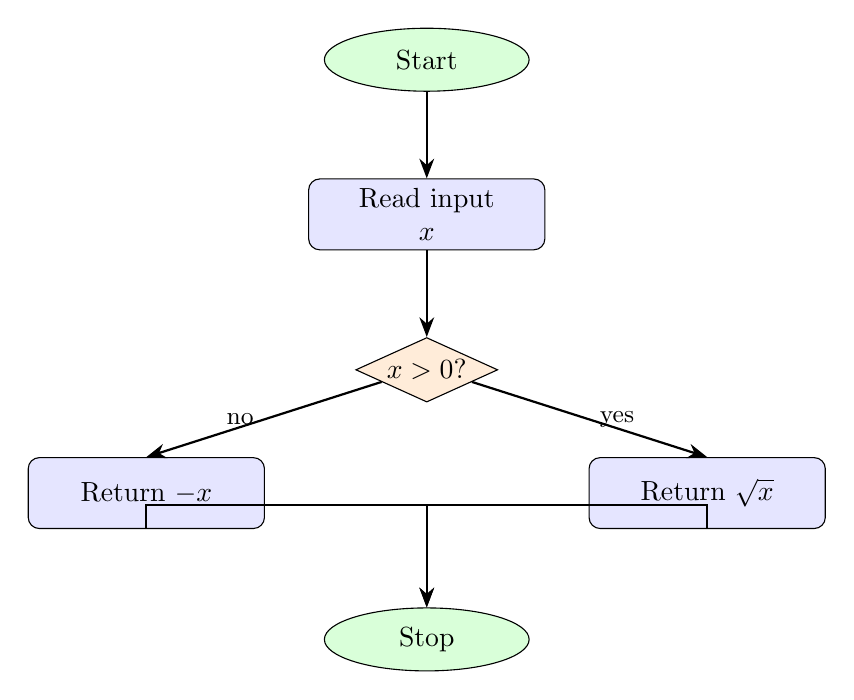
\begin{tikzpicture}[
      node distance=1.1cm and 1.8cm,
      process/.style={rectangle, draw, rounded corners, fill=blue!10, minimum width=3cm, minimum height=0.9cm, align=center},
      decision/.style={diamond, draw, aspect=2.2, fill=orange!15, align=center, inner sep=1pt},
      terminal/.style={ellipse, draw, fill=green!15, minimum width=2.6cm, minimum height=0.8cm},
      flow/.style={-{Stealth[length=2.5mm]}, thick},
    ]
    \node[terminal] (start) {Start};
    \node[process, below=of start] (read) {Read input\\$x$};
    \node[decision, below=of read] (check) {$x > 0$?};
    \node[process, below left=0.9cm and 1.6cm of check] (neg) {Return $-x$};
    \node[process, below right=0.9cm and 1.6cm of check] (pos) {Return $\sqrt{x}$};
    \node[terminal, below=2.6cm of check] (stop) {Stop};

    \draw[flow] (start) -- (read);
    \draw[flow] (read) -- (check);
    \draw[flow] (check.195) -- node[left, font=\small] {no} (neg.north);
    \draw[flow] (check.345) -- node[right, font=\small] {yes} (pos.north);
    \draw[flow] (neg.south) |- ($(check.south)+(0,-1.3cm)$) -- (stop);
    \draw[flow] (pos.south) |- ($(check.south)+(0,-1.3cm)$) -- (stop);
  \end{tikzpicture}
\end{center}

\section{Graph}

\begin{center}
  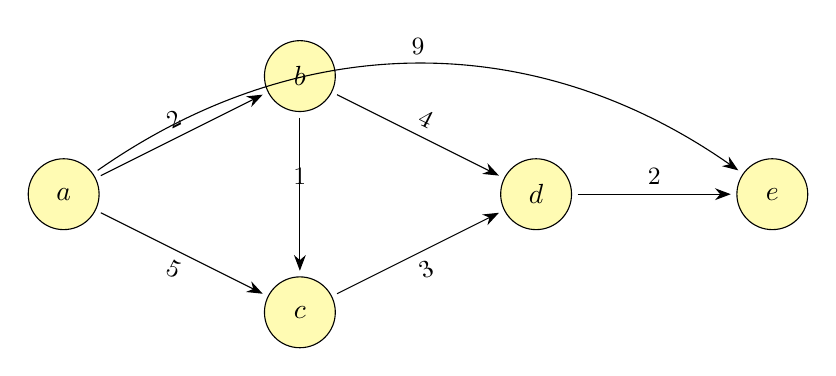
\begin{tikzpicture}[
      vertex/.style={circle, draw, fill=yellow!30, minimum size=0.9cm, inner sep=0pt},
      edge/.style={-{Stealth[length=2mm]}, shorten >=2pt, shorten <=2pt},
    ]
    \node[vertex] (a) at (0,0)   {$a$};
    \node[vertex] (b) at (3,1.5) {$b$};
    \node[vertex] (c) at (3,-1.5) {$c$};
    \node[vertex] (d) at (6,0)   {$d$};
    \node[vertex] (e) at (9,0)   {$e$};

    \draw[edge] (a) -- node[above, sloped, font=\small] {2} (b);
    \draw[edge] (a) -- node[below, sloped, font=\small] {5} (c);
    \draw[edge] (b) -- node[above, font=\small] {1} (c);
    \draw[edge] (b) -- node[above, sloped, font=\small] {4} (d);
    \draw[edge] (c) -- node[below, sloped, font=\small] {3} (d);
    \draw[edge] (d) -- node[above, font=\small] {2} (e);

    \draw[edge, bend left=35] (a) to node[above, font=\small] {9} (e);
  \end{tikzpicture}
\end{center}

\end{document}
